\documentclass[10pt]{article}
\usepackage[utf8]{inputenc}
\usepackage[swedish]{babel}

\def\doctitle{Stadga}
\def\antagen{1997-11-10}
\def\uppdaterad{2016-04-20}

\usepackage{../e-styrdok}
\usepackage{../../e-sek}

\setcounter{tocdepth}{1}
\titleformat{\section}{\bf \Large}{Kapitel {\thetitle} -- }{0mm}{}
\renewcommand{\thesubsection}{\S \arabic{section}:\arabic{subsection}}
\renewcommand{\thesubsubsection}{\S \arabic{section}:\arabic{subsection}:\arabic{subsubsection}}
%\setlength\cftbeforesecskip{0em}

\begin{document}
\firstpage{Stadgar för E-sektionen inom TLTH}{\uppdaterad}
\newpage

\tableofcontents
\newpage

%Kapitel 1
\section{Sektionen}
\subsection{Namn}
E-sektionen inom Teknologkåren vid Lunds Tekniska Högskola, i
dessa Stadgar kallad sektionen.

En kortare benämning är E-sektionen inom TLTH eller bara E-sektionen.
\subsection{Ändamål}
Föreningens ändamål är att främja medlemmarnas studier och utbildning samt
vad därmed äger sammanhang.

Sektionen drivs utan vinstintresse.
\subsection{Emblem}
Sektionens officiella emblem är ``krusidull-E't'' samt ``run-E't'' med
utseende enligt figur 1 och 2,
\begin{figure}[h!tbp]
    \centering
    \parbox{0.3\textwidth}{%
    
\includegraphics[width=0.3\textwidth]{krusidull}
    \caption{``krusidull-E't''}%
    \label{fig:2figsA}}%
    \qquad
    \begin{minipage}{0.3\textwidth}%
        
\includegraphics[width=\textwidth]{rune}
        \caption{``run-E't''}%
        \label{fig:2figsB}%
    \end{minipage}%
\end{figure}%
\subsection{Färg}
Sektionens officiella färg är vit.
\subsection{Maskot}
Sektionens officiella maskot är Hacke Hackspett.
\subsection{Djur}
Sektionens officiella djur är hackspett.
\subsection{Rätt}
Sektionens officiella rätt är klägg eller vegetarisk dito.
\subsection{Träd}
Sektionens officiella träd är trädet på ön Ön.
\subsection{Blomma}
Sektionens officiella blomma är Eldewei\ss.
\subsection{Hedersstuderande}
Sektionens ende hedersstuderande är Oddput Clementin E-62
\newpage

%Kapitel 2
\section{Medlemmarna}
\subsection{Ordinarie medlem}
\subsubsection{Definition}
Ordinarie medlem är varje studerande vid
\begin{dashlist}
\item Civilingenjörsutbildningen i Elektroteknik, LTH,
\item Civilingenjörsutbildningen i Medicin och teknik, LTH,
\item Mastersprogrammet System på chips, LTH, samt
\item Mastersprogrammet Trådlös kommunikation, LTH,
\end{dashlist}
som fullgjort sina skyldigheter gentemot TLTH enligt TLTH:s stadgar §2:1 och §2:2.

\subsubsection{Skyldigheter}
Ordinarie medlem är skyldig att iaktta sektionens
Stadgar och Reglemente.

\subsubsection{Rättigheter}
Medlem som har fullgjort sina skyldigheter enligt
§2:1:1 äger rätt

\begin{attlist}
\item med en röst deltaga i sektionens allmänna val och omröstningar,
\item kandidera till sektionens funktionärsposter,
\item deltaga vid Sektionsmöte och stormöten-SRE, med rösträtt, yrkanderätt
    och yttranderätt,
\item få en viss fråga behandlad av Styrelsen,
\item taga del av sektionens protokoll och handlingar,
\item erhålla av sektionen utgivna publikationer, samt
\item delta i sektionens övriga allmänna aktiviteter.
\end{attlist}


\subsection{Förutvarande medlem}
\subsubsection{Definition}
Med förutvarande medlem avses en person som tidigare varit ordinarie medlem.

\subsubsection{Skyldigheter}
Förutvarande medlem är skyldig att iaktta sektionens Stadgar och Reglemente
då personen önskar delta i sektionens aktiviteter.

\subsubsection{Rättigheter}
Förutvarande medlem som uppfyllt sina skyldigheter
enligt §2:2:2 äger rätt
\begin{attlist}
\item kandidera till sektionens alla funktionärsposter, undantaget ledamot av
    Styrelsen och valberedningens ordförande, samt de i
    Reglementet undantagna funktionärsposterna.
\item deltaga vid Sektionsmöte, med yrkanderätt och yttranderätt,
\item få en viss fråga behandlad av Styrelsen,
\item taga del av sektionens protokoll och handlingar, samt
\item delta i sektions allmänna övriga aktiviteter, men ej i beslut.
\end{attlist}

\subsection{Hedersmedlem}
\subsubsection{Definition}
Med hedersmedlem avses en person som blivit utnämnd enl. §2:3:2.

\subsubsection{Utnämnande}
Hedersmedlem utses av Sektionsmötet med 9/10 majoritet av samtliga avgivna
röster vid sluten omröstning.

Om förslaget faller införes varken förslag eller beslut i protokoll.

\subsubsection{Skyldigheter}
Hedersmedlem är skyldig att iaktta sektionens Stadgar och Reglemente då
personen önskar delta i sektionens aktiviteter.

\subsubsection{Rättigheter}
Som sådan äger man rätt att deltaga i sektionens allmänna aktiviteter men ej
i sektionens beslut.
\newpage

%Kapitel 3
\section{Organisation}
\subsection{Organisationsplan}
Sektionen är organiserad i enlighet med organisationsplanen i figur~3.
\begin{figure}[h!tbp]
    \centering
    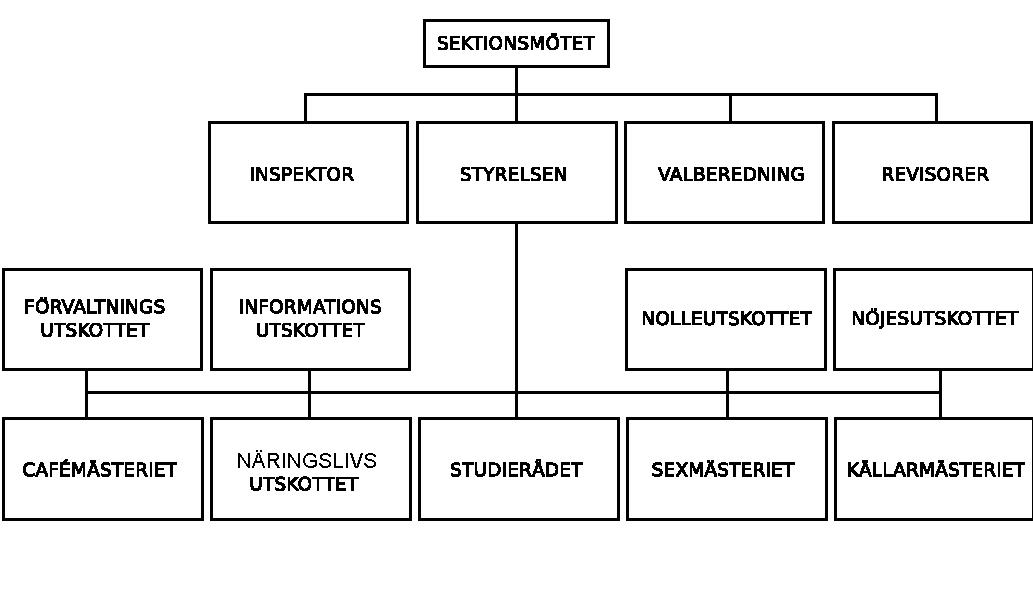
\includegraphics[width=0.9\textwidth]{orgplan}
    \caption{``Organisationsplan''}%
    \label{fig:orgplan}%
\end{figure}%
\newpage

%Kapitel 4
\section{Sektionsmöte}
\subsection{Befogenhet}
Sektionsmötet är sektionens högsta beslutande organ.

\subsection{Rösträtt}
Rösträtt tillkommer sektionens ordinarie medlemmar.

\subsection{Beslutsförhet}
Sektionsmötet äger rätt att fatta beslut om, och endast om, antalet
närvarande röstberättigade är tjugoen (21) eller fler, dock skall ej Styrelsen
vara i majoritet.

\subsection{Solidaritet}
Närvarande röstberättigad medlem som utan reservation deltagit i beslut som
fattats av Sektionsmötet är solidariskt ansvarig för detta.

\subsection{Reservation}
Reservation mot beslut, skriftlig eller blank, skall anmälas till
mötesordföranden innan mötespunkten avslutas.

I de fall då reservationen är skriftlig skall den lämnas in till
mötessekreteraren senast 24 timmer efter det att mötet avslutats.

\subsection{Röstning}
Vid röstning på Sektionsmöte får ej fullmakt avgivas.

\subsection{Adjungering}
Sektionsmötet äger rätt att adjungera personer till mötet.

Adjungerad person har yttrande- och yrkanderätt.

\subsection{Ständigt adjungerade}
Ständigt adjungerade med yttrande och yrkanderätt på
Sektionsmöte är
\begin{alphlist}
\item 	revisorerna,
\item 	inspektorn,
\item 	representant ifrån TLTH:s styrelse, samt
\item 	övriga enligt Reglemente.
\end{alphlist}

\subsection{Ordinarie Sektionsmöte}
Under året skall tre (3) ordinarie Sektionsmöten hållas,
\begin{alphlist}
\item 	Vårterminsmöte,
\item 	Höstterminsmöte, som gemensamt benämns Terminsmöte, samt
\item 	Valmöte, som hålls på hösten.
\end{alphlist}

\subsection{Vårterminsmötet}
Vid Vårterminsmötet skall följande ärenden tas upp:
\begin{alphlist}
\item 	val av funktionärer enligt Reglemente,
\item 	verksamhetsberättelse för föregående verksamhetsår,
\item 	bokslut för föregående verksamhetsår,
\item 	revisorernas berättelse för samma tid,
\item 	resultatdisposition,
\item 	frågan om ansvarsfrihet för:
    \begin{numplist}
        \item  	funktionärer,
        \item 	Utskotten,
        \item 	Styrelsen,
        \item 	Revisorerna, samt
        \item 	Valberedningen.
    \end{numplist}
\item 	motioner inlämnade i rätt tid enl. §4:14, samt
\item 	de punkter som föreskrivs i Reglementet.
\end{alphlist}

\subsection{Höstterminsmötet}
Vid Höstterminsmötet skall följande ärenden tas upp:
\begin{alphlist}
\item 	budget inför kommande verksamhetsår,
\item 	resultatrapport från första halvan av verksamhetsåret,
\item 	revision av utskottsbeskrivningar,
\item 	motioner inlämnade i rätt tid enl. §4:14, samt
\item 	de punkter som föreskrivs i Reglementet.
\end{alphlist}

\subsection{Valmötet}
Vid Valmötet skall endast följande ärenden tas upp:
\begin{alphlist}
\item val av Styrelse och funktionärer enligt Reglemente,
\item val av Valberedning,
\item val av Revisorer,
\item val av representanter till TLTH:s utskott enligt gällande Stadgar och
    Reglemente för TLTH, samt
\item övriga valärenden enligt Reglementet.
\end{alphlist}

\subsection{Utlysande}
Kallelse till ordinarie Sektionsmöte skall av Styrelsen uppsättas på
sektionens anslagstavla senast elva (11) läsdagar före Sektionsmötet, samt
delges Inspektorn och Revisorerna.

Kallelse till extra Sektionsmöte skall på samma sätt offentliggöras senast
sju (7) läsdagar före mötet.

Sektionsmöte måste hållas på läsdag.

Kallelse till två (2) Sektionsmöten, undantaget Sektionsmötet i kombination
med Valmötet, får ej föreligga samtidigt.

Valmötet får ej hållas före Höstterminsmötet, ej heller samma dag.

Föredragningslista, med tillhörande handlingar, till Sektionsmöte skall
uppsättas på sektionens anslagstavla senast fem (5) läsdagar före mötet.

\subsection{Upptagande av motion}
Varje medlem äger rätt att taga upp fråga på Terminsmöte.
Sådan motion skall skriftligen ha inkommit till Styrelsen senast åtta (8)
läsdagar innan Terminsmötet.

\subsection{Extra Sektionsmöte}
Extra Sektionsmöte skall hållas då

\begin{alphlist}
\item Styrelsen så kräver,
\item Inspektorn så kräver,
\item Revisorerna så kräver, eller
\item minst tjugofem (25) ordinarie medlemmar skriftligen därom anhåller
    och med uppgivande av vilket eller vilka ärenden som önskas behandlas.
\end{alphlist}

Extra Sektionsmöte skall hållas tio (10) läsdagar efter det att anhållan
inkommit till Styrelsen.

Härvid får inte §4:13 överträdas.

\subsection{Ajournering}
Sektionsmöte må med enkel majoritet besluta att ajournera mötet och där vid
fastställa tidpunkten för mötets återupptagande.

Om Sektionsmötet återupptas först kommande läsdag eller senare skall
meddelande därom snarast anslås på sektionens anslagstavla.

Sektionsmötet får ej ajourneras i mer än sju (7) läsdagar eller över
terminsskifte.

Om Sektionsmötet av någon anledning ej kan återupptas vid utsatt tidpunkt,
gäller det som vid tidpunkten för ajourneringen beslutats och mötet är
avslutat.
\newpage

%Kapitel 5
\section{Inspektor}
\subsection{Inspektor}
Inspektorn skall ägna uppmärksamhet åt och stödja sektionens verksamhet.

\subsection{Valbarhet}
Inspektorn skall vara lärare verkande vid LTH.

Inspektorn väljs på ett Sektionsmöte.

\subsection{Mandattid}
Inspektorns mandattid är två (2) år med börja vid halvårsskiftet.

\subsection{Skyldigheter}
Inspektorn är skyldig:
\begin{attlist}
\item hålla sig informerad om sektionens verksamhet, samt
\item verka för ett gott förhållande mellan sektionen och högskolan i övrigt.
\end{attlist}

\subsection{Rättigheter}
Inspektorn äger rätt:
\begin{attlist}
\item  	erhålla kallelse, handlingar och protokoll från Sektionsmöte,
\item 	erhålla kallelse och protokoll från Styrelsens sammanträde,
\item 	närvara med yttrande och yrkanderätt vid sektionens myndigheters
    sammanträden utom vid Valberedningens sammanträde,
\item  	kalla till extra Sektionsmöte och extra sammanträde för Styrelsen, samt
\item  	erhålla av sektionen utgivna publikationer.
\end{attlist}
\newpage

%Kapitel 6
\section{Revision}
\subsection{Uppgift}
Revisorerna skall i den omfattning som följer av god revisionssed granska
föreningens årsredovisning jämte räkenskaperna samt Styrelsens förvaltning.

\subsection{Sammansättning}
Revisorerna skall vara två (2) till antalet.

Minst en skall dessutom äga god insikt i sektionens verksamhet.

Revisorsuppleanterna skall vara två (2) till antalet.

\subsection{Krav}
Revisorerna och Revisorsuppleanterna skall vara myndiga, samt ha den insikt i
ekonomiska förhållanden som uppdraget kräver.

Revisorerna och Revisorsuppleanterna får ej ha andra förtroendeuppdrag inom
sektionen.

\subsection{Mandattid}
Revisorernas och Revisorsuppleanternas mandattid är kalenderår.

\subsection{Rättigheter}
Revisorerna äger rätt
\begin{attlist}
\item närhelst de önskar taga del av samtliga räkenskaper, protokoll och
    andra handlingar, samt äga tillträde till sektionens lokaler,
\item begära och erhålla upplysningar rörande verksamhet och förvaltning,
\item erhålla kallelse, handlingar och protokoll från Sektionsmöte,
\item erhålla kallelse och protokoll från Styrelsens sammanträde,
\item närvara med yttrande och yrkanderätt vid sektionens myndigheters
    sammanträden utom vid Valberedningens sammanträde,
\item kalla till extra Sektionsmöte och extra sammanträde för Styrelsen, samt
\item erhålla av Sektionen utgivna publikationer.
\end{attlist}

\subsection{Skyldigheter}
Revisorerna är skyldiga
\begin{attlist}
\item hålla sig informerad om Sektionens verksamhet,
\item senast sju (7) läsveckor efter verksamhetsårets slut inlämna
    revisionsberättelse, samt på balansräkningen ha tecknat påskrift med
    yttrande huruvida dessa handlingar överensstämmer med Sektionens böcker,
    samt
\item skriftligen meddela Styrelsen då någon av dem ej längre kan fullgöra
    sitt uppdrag som Revisor.
\end{attlist}

\subsection{Revisionsberättelse}
Revisionsberättelse skall innehålla särskilt yttrande angående
\begin{alphlist}
\item fastställande av balansräkningen,
\item ansvarsfrihet för Styrelsen, samt
\item Styrelsens förslag till resultatdisposition.
\end{alphlist}
\newpage

%Kapitel 7
\section{Valberedning}
\subsection{Uppgift}
Valberedningen har till uppgift att förbereda val som skall förrättas av
Sektionsmöte.

\subsection{Sammansättning}
Valberedningen består av:
\begin{alphlist}
\item Ordförande,
\item en sekreterare,
\item två (2) ledamöter,
\item en (1) representant ur Nolleutskottet,  samt
\item en (1) av Valberedningen utsedd representant bland de nyinskrivna.
\end{alphlist}

Valberedningens Ordförande får inte sitta med i Styrelsen eller bli nominerad till någon av dessa poster.

Ledamot av Valberedningen får ej nomineras till poster i Styrelsen.

\subsection{Mandattid}
För valberedningen är mandattiden kalenderår.

\subsection{Skyldigheter}
Det åligger sektionens Valberedning att senast åtta (8) läsdagar före
sektionens Valmöte och Vårterminsmöte för Styrelsen framlägga förslag till
val i enlighet med §12:2, samt vad som föreskrivs i Reglementet.

I och med att Styrelsen tagit del av Valberedningens förslag är detta
offentligt, och skall uppsättas på sektionens anslagstavla.
\newpage

%Kapitel 8
\section{Styrelsen}
\subsection{Befogenhet}
Styrelsen är sektionens högsta verkställande organ.

\subsection{Sammansättning}
Styrelsen består av
\begin{alphlist}
\item Ordförande,
\item studierådsordförande, tillika utskottsordförande för Studierådet,
\item sekreterare, tillika utskottsordförande för Informationsutskottet,
\item kassör, tillika utskottsordförande för Förvaltningsutskottet, samt
\item sex ledamöter, tillika utskottsordföranden för Nolleutskottet,
    Nöjesutskottet, Cafémästeriet, Källarmästeriet, Sexmästeriet och
    Näringslivsutskottet.
\end{alphlist}

Benämning på ledamöterna i Styrelsen enligt c-e fastställs av Reglementet.

Styrelsen utser inom sig en vice ordförande.

\subsection{Krav}
Ledamot av Styrelsen skall vara myndig och ordinarie medlem av Sektionen,
samt ha den insikt i styrelseposten som uppdraget kräver.

\subsection{Mandattid}
För Styrelsen är mandattiden kalenderår.

\subsection{Sammanträde}
Styrelsen sammanträder på kallelse av Ordföranden, dock minst tre (3) gånger
per termin, samt i övrigt då Revisorer, Inspektorn eller någon annan i
Styrelsen så kräver.

\subsection{Beslut}
Styrelsen är beslutsmässig om minst sex (6) ledamöter är närvarande.

Vid lika röstetal äger Ordföranden utslagsröst.

\subsection{Adjungering}
Styrelsen äger rätt att adjungera personer till Styrelsens sammanträden.

\subsection{Ständigt adjungerade}
Ständigt adjungerade med yttrande och yrkanderätt
vid Styrelsens sammanträden är

\begin{alphlist}
\item Revisorerna,
\item Inspektorn,
\item representant ur TLTH:s styrelse, samt
\item övriga enligt Reglemente.
\end{alphlist}

\subsection{Kallelse}
Kallelse till Styrelsens sammanträde, samt föredragningslista skall senast
tre (3) läsdagar före sammanträdet tillställas

\begin{alphlist}
\item Styrelsens ledamöter,
\item Revisorerna,
\item Inspektorn,
\item TLTH:s styrelse, samt
\item övriga enligt Reglemente.
\end{alphlist}

samt dessutom anslås på sektionens anslagstavla.

\subsection{Särskild kallelse}
Under sommaruppehållet skall kallelse till Styrelsens sammanträde, samt
föredragningslista utgå via e-post senast elva (11) vardagar före sammanträdet.

\subsection{Skyldigheter}
Det åligger Styrelsen
\begin{attlist}
\item inför sektionsmötet ansvara för sektionens hela verksamhet,
\item förbereda och genomföra Sektionsmöten,
\item verkställa och övervaka genomförandet av Sektionsmötets beslut,
\item tillse att gällande Stadgar, Reglemente och föreskrifter för
    Sektionen efterlevs,
\item ansvara för sektionens medel,
\item till Höstterminsmötet framlägga förslag till budget,
\item verkställa fortlöpande inventering av sektionens kassa och övriga
    tillgångar,
\item bereda inkomna förslag, handha sektionens korrespondens samt i övrigt
    sköta löpande ärenden,
\item senast tre (3) läsveckor efter verksamhetsårets slut till Revisorerna
    överlämna Styrelsens och Utskottens verksamhetsberättelser, protokoll,
    bokslut och övriga handlingar,
\item handlägga fyllnadsval i enlighet med §12:3, samt
\item även i övrigt på alla sätt verka för sektionens bästa.
\end{attlist}


\subsection{Solidaritet}
Ledamot av Styrelsen som utan reservation deltagit i beslut som fattats i
Styrelsen är solidariskt ansvarig för detta.

Ledamot av Styrelsen som ej varit närvarande vid beslut, är solidariskt
ansvarig, om ledamoten inte reserverat sig i protokollet senast vid nästa
sammanträde för Styrelsen.
\newpage

%Kapitel 9
\section{Utskott}
\subsection{Definition}
Sektionens Utskott är:
\begin{alphlist}
\item Förvaltningsutskottet, FVU,
\item Informationsutskottet, InfU,
\item Näringslivsutskottet, ENU,
\item Nöjesutskottet, NöjU,
\item Källarmästeriet, KM,
\item Cafémästeriet, CM,
\item Sexmästeriet, E6,
\item Nolleutskottet, NollU, samt
\item Studierådet, SRE.
\end{alphlist}

\subsection{Skyldigheter}
Det åligger sektionens Utskott
\begin{attlist}
\item följa gällande Stadgar och Reglemente, samt
\item verkställa av Styrelsen eller Sektionsmöte fattade beslut.
\end{attlist}
Det åligger utskottsordförande
\begin{attlist}
\item leda och fördela arbetet inom Utskottet,
\item budgetera, redovisa och följa upp Utskottets verksamhet, samt
\item senast två (2) läsveckor efter verksamhetsårets slut till Styrelsen
    inlämna verksamhetsberättelse.
\end{attlist}

\subsection{Sammansättning}
Varje Utskott består av
\begin{alphlist}
\item utskottsordförande, tillika ledamot av Styrelsen, samt
\item funktionärer enligt Reglementet.
\end{alphlist}

\subsection{Förvaltningsutskottet, FVU}
Det åligger Förvaltningsutskottet att förvalta sektionens ekonomi,
lokaler och inventarier.

\subsection{Informationsutskottet, InfU}
Det åligger Informationsutskottet att tillgodose medlemmarnas
intressen frågor som berör information och marknadsföring.

Informationsutskottet ansvarar även för verksamheten i de redaktionella
organen.

\subsection{Näringslivsutskottet, ENU}
Det åligger Näringslivsutskottet att skapa och
sköta kontakter mot industri och företag för medlemmarnas räkning.

Det åligger Näringslivsutskottet att tillgodose
sektionens behov av sponsring.

\subsection{Nöjesutskottet, NöjU}
Det åligger Nöjesutskottet att tillgodose sektionens medlemmar med
nöjes- fritids- och idrottsarrangemang.

\subsection{Källarmästeriet, KM}
Det åligger Källarmästeriet att anordna pubar och gillen med tillhörande mat
och dryckförsäljning.

\subsection{Cafémästeriet, CM}
Det åligger Cafémästeriet att sköta caféförsäljningen i LED-café samt att i Edekvata tillhandahålla försäljning via mojter.

\subsection{Sexmästeriet, E6}
Det åligger Sexmästeriet att tillgodose sektionens medlemmar med
festarrangemang.

\subsection{Nolleutskottet, NollU}
Det åligger Nolleutskottet att planera och genomföra mottagandet av
de nyinskrivna, både vad gäller fadderverksamhet och nollning.

\subsection{Studierådet, SRE}
\subsubsection{Sammansättning}
Studierådet består av
\begin{alphlist}
\item studierådsordförande,
\item vice studierådsordförande,
\item sekreterare, samt
\item funktionärer enligt Reglementet.
\end{alphlist}


\subsubsection{Mandattid}
För studierådet är mandattiden 1/7-30/6 för utom studierådets ordförande.

Representanter i högskolans organ har den mandattid som respektive organ
fastställt.

\subsubsection{Skyldigheter}
Det åligger Studierådet att sköta utbildningbevakningen och representationen
i högskolans upprättade organ, samt vad som där äga sammanhang.

\subsubsection{Stormöte-SRE}
Minst en (1) gång per läsår skall Studierådet hålla ett Stormöte-SRE.

Till Stormötet-SRE har alla sektionens medlemmar rätt att närvara med
yttrande och yrkanderätt.

Rösträtt tillkommer dem som uppfyller §2:1:1.

\subsubsection{Utlysande}
Kallelse och föredragningslista till Stormöte-SRE skall av Studierådet
uppsättas på sektionens anslagstavla senast elva (11) läsdagar före
Stormötet-SRE.

Möteshandlingar skall finnas tillgängliga på sektionens anslagstavlor senast
fem (5) läsdagar innan mötet.
\newpage

%Kapitel 10
\section{Funktionär}
\subsection{Definition}
Med funktionär avses person som har förtroendeuppdrag inom Sektionen.

\subsection{Mandattid}
En funktionärs mandattid fastställs av Reglementet, om inte Stadgar säger
annat.

\subsection{Skyldighet}
Det åligger sektionens funktionärer
\begin{attlist}
\item följa gällande Stadgar och Reglemente,
\item i största möjliga mån närvara vid Sektionsmöte, samt
\item även i övrigt på alla sätt verka för sektionens bästa.
\end{attlist}

\subsection{Rättighet}
En funktionär har rätt till de förmåner som föreskrivs i Reglementet.
\newpage

%Kapitel 11
\section{Redaktionella organ}
\subsection{Inrättande}
Redaktionella organ må inrättas av Sektionsmötet.

\subsection{Ansvar}
Ansvarig utgivare för de redaktionella organen är utskottsordföranden för Informationsutskottet.

\subsection{HeHE}
Oavsett vad som eljest stadgats gäller för Hent i Hus E:

\subsubsection{Redaktion}
HeHE-redaktionen består av
\begin{alphlist}
\item Chefredaktören, samt
\item ett antal redaktörer enligt Reglementet.
\end{alphlist}

\subsubsection{Mandattid}
För HeHE-redaktionen är mandattiden kalenderår.

\subsubsection{Uppgift}
HeHE:s uppgift är

\begin{attlist}
\item följa gällande Stadgar och Reglemente,
\item förmedla aktuell information om sektionens verksamhet, samt
\item nå ut till alla sektionens ordinarie medlemmar och Inspektor samt
    Revisorer.
\end{attlist}

\subsection{Elskaren}
Elskaren är sektionens tidning.

Elskaren skall utkomma i sådan omfattning som anges i Reglementet.

\subsection{WWW}
WWW är sektionens sidor tillgängliga genom internet.

Dessa sidor jämställs med övriga redaktionella organ inom Sektionen.
\newpage

%Kapitel 12
\section{Val}
\subsection{Valbarhet}
Valbar till ledamot av Styrelsen och till Ordförande av Valberedningen är envar myndig svensk medborgare och ordinarie medlem av Sektionen.

Valbar som Inspektor är envar lärare verkande vid LTH.

Valbar som Revisor eller Revisorsuppleant är de som uppfyller kraven i §6:3.

Valbar som funktionär är ordinarie medlem och då Reglementet ej föreskriver
annorlunda även förutvarande medlemmar av Sektionen.

I de fall då uppdragets art så kräver skall samhällets åldersgränser beaktas.

\subsection{Val}
Sektionsmötets val av Styrelse, Revisorer och
Revisorsuppleanter, Inspektor, Valberedning och funktionärer förbereds av
Valberedningen.

Utöver Valberedningens förslag må fri kandidatnominering ske intill tiden
för frågans avgörande.

\subsection{Fyllnadsval}
Ledamot av Styrelsen, Inspektor, Revisorer och Revisorsuppleanter och
Ordförande av Valberedningen kan endast väljas på
Sektionsmöte.

Fyllnadsval av övriga funktionärer kan förrättas av Styrelsen, om
Reglementet ej föreskriver annorlunda.

\subsection{Avsättandet}
Förtroendevald person kan endast avsättas av Sektionsmötet.

Fram till tiden för frågans avgörande kan Styrelsen, om de anser det
nödvändigt, utse en tillförordnad funktionär att ta över funktionärsysslan.

Sektionsmöte skall hållas inom tio (10) läsdagar från tillförordnandet.

\subsection{Högskoleorgan}
Representanter i högskolans organ nomineras av Stormöte-SRE.

Nominering av representanter förbereds av Studierådet.

Fyllnadsnominering görs av Studierådet.

\subsection{Votering}
Votering är öppen när sluten votering ej begärts.

Där ej annat stadgats eller Reglementet föreskriver annorlunda gäller enkel
majoritet.

Om rösterna är lika fördelade vinner Styrelsens förslag.

I de fall Styrelsen ej har förslag har Ordföranden av Sektionen utslagsrösten.

Votering i personval är alltid sluten och vid lika antal röster avgör lotten.

Röstningsprocedurer enligt Reglementet.
\newpage

%Kapitel 13
\section{Protokoll}
\subsection{Sektionsmöte}
Vid Sektionsmöte förs beslutsprotokoll.

Protokollet skall även ange antalet närvarande vid mötets början och slut.

Protokollet justeras senast tio (10) läsdagar efter mötet av
mötesordföranden samt två (2) på mötet valda justeringspersoner.

\subsection{Övriga sammanträde}
Över besluten vid sammanträden för Styrelsen, Studierådet och
Valberednings föres protokoll med förteckning över de närvarande vid
sammanträdets början och slut.
Sådant protokoll justeras av sammanträdets ordförande och en (1) på mötet
vald justeringsperson inom åtta (8) läsdagar efter sammanträdet.

\subsection{Offentliggörande}
I §13:1 och §13:2 nämnda protokoll skall sedan de justerats finnas
tillgängliga på sektionens anslagstavla och webbplats.
\newpage

%Kapitel 14
\section{Ekonomi}
\subsection{Ekonomi}
Sektionens ekonomi handhas av Förvaltningsutskottet.

\subsection{Verksamhetsår}
Sektionens verksamhetsår och räkenskapsår är kalenderår.

\subsection{Sektionens firma}
Sektionens firma tecknas av sektionsstyrelsen eller av sektionsordförande och kassör i förening.

\subsection{Fonder}
Sektionens fonder är
\begin{alphlist}
\item dispositionsfonden,
\item olycksfonden,
\item utrustningsfonden, samt
\item övriga fonder enligt Reglementet.
\end{alphlist}

Till dispositionsfonden skall årligen enligt Sektionsmötets beslut avsättas
medel tillräckliga för att sektionens verksamhet skall kunna hållas på en
acceptabel nivå.

\subsection{Disposition}
Styrelsen äger rätt att disponera de i dispositionsfonden och olycksfonden
avsatta medlen.

Utrustningsfonden disponeras av Sektionsmötet.

Övriga fonder disponeras enligt Reglementet.

\subsection{Jävighet}
Vid beslut om ansvarsfrihet får de ansvariga inte delta i beslutet.

Inte heller får någon som äger ett personligt ekonomiskt intresse i en
fråga delta i beslutet.
\newpage

%Kapitel 15
\section{Stadgarna}
\subsection{Tolkning}
Vid tolkning av Stadgarna gäller Inspektors åsikt intill dess Sektionsmötet
beslutat i saken.

\subsection{Ändring}
Förslag till stadgeändring inlämnas till Styrelsen senast åtta (8) läsdagar
före Terminsmöte.

Förslaget offentliggörs senast fem (5) läsdagar innan Terminsmötet.

För slutgiltigt bifall fordras likalydande beslut med minst 2/3 majoritet på
två (2) på varandra följande Terminsmöten.

\subsection{Giltighet}
Dessa Stadgar är ej giltiga förrän de fastställts av Teknologkårens
Fullmäktige.
\newpage

%Kapitel 16
\section{Reglemente}
\subsection{Definition}
Reglemente är ett tillägg till Stadgarna, i vilket tillämpningsföreskrifter,
utskottsbeskrivningar, policybeslut och övriga föreskrifter återfinns.

\subsection{Utskottsbeskrivning}
En utskottsbeskrivning är en föreskrift om Utskottets funktionärer med
tillhörande åligganden, samt Utskottets arbetsuppgifter.

\subsection{Policybeslut}
Ett policybeslut är en föreskrift i en speciell fråga som Terminsmötet har
tagit beslut om.

\subsection{Ändring}
Ändring kan endast ske med
\begin{alphlist}
\item 2/3 majoritet på ett Terminsmöte, eller
\item enkel majoritet vid två (2) på varandra följande Terminsmöte.
\end{alphlist}

\subsection{Tolkning}
Vid tolkning av Reglementet gäller Styrelsens åsikt intill dess Sektionsmötet
beslutat i saken.

Då Reglementet står i konflikt med Stadgarna, gäller Stadgarna.
\newpage

\section{Upplösning}
\subsection{Upplösning}
Sektionen får ej upplösas.
\newpage

\section*{Interna hänvisningar i stadgan}
\renewcommand*\arraystretch{1}
\begin{tabular}{p{15mm} p{90mm}}
    Paragraf & Hänvisning till Teknologkårens stadga\\
    §2:2:1 & §2:1 och §2:2\\
    &\\
    Paragraf & Hänvisning till Sektionens Stadga\\
    §2:1:3 & §2:1:1\\
    §2:2:3 & §2:2:2\\
    §2:3:1 & §2:3:2\\
    §4:10 & §4:14\\
    §4:11 & §4:14\\
    §4:15 & §4:13\\
    §7:4 & §12:2\\
    §8:11 & §12:3\\
    §9:12:4 & §2:1:1\\
    §12:1 & §6:3\\
    §13:3 & §13:1 och §13:2\\
    &\\
    Paragraf & Hänvisning till Sektionens Reglemente\\
    §2:2:3 & Kapitel 12\\
    §4:8 & Kapitel 4\\
    §4:10 & Kapitel 11\\
    §4:10 & Kapitel 4\\
    §4:11 & Kapitel 4\\
    §4:12 & Kapitel 11\\
    §7:4 & Kapitel 11\\
    §8:2 & Kapitel 8\\
    §8:8 & Kapitel 8\\
    §8:9 & Kapitel 8\\
    §9:3 & Kapitel 11\\
    §9:12:1 & Kapitel 11\\
    §10:2 & Kapitel 11\\
    §10:4 & Kapitel 11\\
    §11:3:1 & Kapitel 11\\
    §11:4 & Kapitel 9\\
    §12:1 & Kapitel 12\\
    §12:3 & Kapitel 12\\
    §12:6 & Kapitel 12\\
    §14:4 & Kapitel 14\\
    §14:5 & Kapitel 14\\
\end{tabular}
\renewcommand*\arraystretch{1.3}

\newpage
\section*{Revidering av stadgan}

\renewcommand*\arraystretch{1}
\begin{tabular}{p{7mm} p{110mm}}
    V1.0 & Stadgan tagen i en andra läsning på Höstterminsmötet 1997-11-10\\
    V1.1 & Stadgan reviderad i en andra läsning på Höstterminsmötet 1998-11-09\\
    & §4:3, §7:3, §9:4\\
    V1.2 & Stadgan reviderad i en andra läsning på Vårterminsmötet 1999-05-10\\
    & Diverse redaktionella ändringar, §4:4, §4:5 \\
    V1.3 & Stadgan reviderad i en andra läsning på Höstterminsmötet 1999-11-08\\
    & §2:2:3, §4:8, §4:9, §4:10, §4:13, §12:1 §12:3\\
    V1.4 & Stadgan reviderad i en andra läsning på Höstterminsmötet 2000-10-30\\
    & §7:2, §4:3, §4:13\\
    V1.5 & Stadgan reviderad i en andra läsning på Höstterminsmötet 2001-11-06\\
    & §4:13\\
    V1.6 & Stadgan reviderad i en andra läsning på Höstterminsmötet 2002-11-14\\
    & §4:10, §4:11, §4:12, §4:13, §4:16, §9:12:4, §11:3:4, §13:3\\
    V1.7 & Stadgan reviderad i en andra läsning på Vårterminsmötet 2003-05-21\\
    & §8:2, §8:10, §9:1:C, §9:6 \\
    V1.8 & Stadgan reviderad i en andra läsning på Vårterminsmötet 2004-05-06\\
    & §1:6. §1:7. §1:8	\\
    V1.9 & Stadgan reviderad i en andra läsning på Vårterminsmötet 2005-05-12\\
    & §1:9\\
    V2.0 & Stadgan reviderad i en andra läsning på Höstterminsmötet 2011-11-09\\
    & §1:1, §2:1, §3:1, §8:2, §9:1, §9:6\\
     V2.1 & Stadgan reviderad i en andra läsning på Vårterminsmötet 2014-04-18\\
    & Reviderat: §2:2:3, §3:1, §4:10, §4:12, §7.2, §8:2, §8:4, §8:11, §9:1, §9:6, §11:2, §11:3:1,
    §11:3:4, §12:1, §12:2, §12:3
    Borttaget: §11:3:3\\
    V2.2 & Stadgan reviderad i en andra läsning på Höstterminsmötet 2015-11-17\\
    V2.3 & Stadgan reviderad i en andra läsning på Vårterminsmötet 2016-04-20\\
\end{tabular}
\renewcommand*\arraystretch{1.3}

För specifikation av ändringar, se Stadgans revideringshistorik.

\section*{Stadgeändringar tagna i en första läsning}

Se Stadgans revideringshistorik

\end{document}
